\providecommand{\StudySection}{\section}
\providecommand{\StudySubsection}{\subsection}

\StudySection{Expanding seeds selectively and using an intermediate basis}
\label{sec:basis-completion}
The graph-specific study identifies symbolic equation regeneration as the largest measured solver stage. Some target batches need seed limits beyond those of the targets themselves, and a general enlargement can generate many unnecessary equations. We therefore test whether selective increases in the limits, or a reduction through an intermediate master basis, can lower this remaining cost.

The candidate set contains six ways to increase selected seed limits and two ways to reduce first to a temporary basis. In the latter case, Kira reduces the remaining temporary masters to the prescribed basis, and exact multiplication combines the two coefficient matrices. The final basis requirement is the same for every method. Appendix~\ref{app:basis-completion} defines the candidates and derives this conversion, which allows the first target reduction to use a smaller system when the remaining basis conversion is inexpensive.

For development batch $c$, let $B_c=(r_c,s_c,q_c)$ denote valid initial limits on the positive index sum, numerator rank, and number of extra denominator powers. We retain the fastest new candidate for a development batch only if it saves at least ten percent against the graph-specific method in Section~\ref{sec:type-specialists}. The resulting candidate set contains that preceding method, full-sector basis completion, and the selective increments $B_c+(1,0,0)$, $B_c+(0,1,0)$, and $B_c+(1,1,0)$. Development results select the options but do not enter the reserved comparison.

The new data contain 36 training batches, 18 validation batches, and 36 test batches from the same seven graphs and target patterns, with new rational kinematics and symbolic $d$. Ten predictors per graph use the same nine features to predict time relative to the preceding method. Validation compares each predictor with that method and with a fixed new strategy selected from training for each graph. A predictor is enabled only if it saves at least five percent against the faster control; otherwise that control is used. A fixed candidate may itself call the preceding learned method, so this comparison tests the additional choice among the new options.

Validation enables new predictors for three graphs. The retained training and validation records contain 1,731.7 seconds of measured reductions, and fitting the seventy candidates takes 0.88 seconds. These costs exclude reference construction and development and remain outside the reserved reduction timer.

The test compares native choices, the preceding graph-specific method, the new fixed strategy, and the selected strategy. Five repetitions give 720 calculations, all of which pass exact checks. A further 43 applications also pass when the reduction receives no target reference coefficients. With equal weight for each graph, the selected method has ratio $0.9115$ to the preceding method, with descriptive interval $[0.8105,0.9980]$, giving 8.8\% less time. Its ratio to native choices in the same experiment is $0.8516$ with interval $[0.7282,0.9647]$, giving 14.8\% less time. Relative to the new fixed strategy, the ratio is $0.9264$ with interval $[0.8760,0.9747]$.

The sum of batch medians answers a different question: how long would this set of requests take when each is counted once? For the 36 reserved batches, this sum is 106.24 seconds for native choices, 96.32 seconds for the preceding method, and 77.03 seconds for the selected method. The geometric ratios above instead give every graph equal weight. Both measures show a saving, although their magnitudes differ because the longer calculations contribute more to the workload total.

The stage measurements explain where part of the saving occurs. Across 180 runs per method, symbolic equation regeneration falls from 138.02 to 80.58 seconds. Neither the preceding nor the selected method makes a fallback attempt, compared with 40 for native choices. Planned second-stage reductions of temporary masters are included in complete time and are counted separately from fallback. The comparison with the fixed strategy supports an additional benefit from the selection procedure, which combines validation-based control choices with predictions for individual target batches.

\begin{table}[!htbp]
\centering\small
\caption{Selective seed expansion compared with the graph-specific method in Section~\ref{sec:type-specialists}. Times are geometric means of batch medians in seconds. ``Previous'' denotes that graph-specific method and ``New'' denotes the seed-expansion method. Each graph has two reserved parameter profiles.}
\label{tab:basis-completion}
\begin{tabular}{@{}llrrrr@{}}\toprule
Graph & Policy & Previous (s) & New (s) & New/previous & New/native\\\midrule
Sunrise & Add $s$ & 0.596 & 0.593 & 0.995 & 0.979\\
Planar box & Tree depth 1 & 2.422 & 2.062 & 0.851 & 0.735\\
Vacuum & Complete basis & 0.928 & 0.941 & 1.013 & 1.016\\
Ladder & Tree depth 1 & 4.477 & 3.007 & 0.672 & 0.584\\
Nonplanar box & Tree depth 1 & 4.091 & 3.550 & 0.868 & 0.759\\
Pentagon & Previous & 0.723 & 0.754 & 1.043 & 0.998\\
Virtuality box & Previous & 0.580 & 0.582 & 1.003 & 1.004\\
\bottomrule\end{tabular}
\end{table}

\begin{figure}[!htbp]
\centering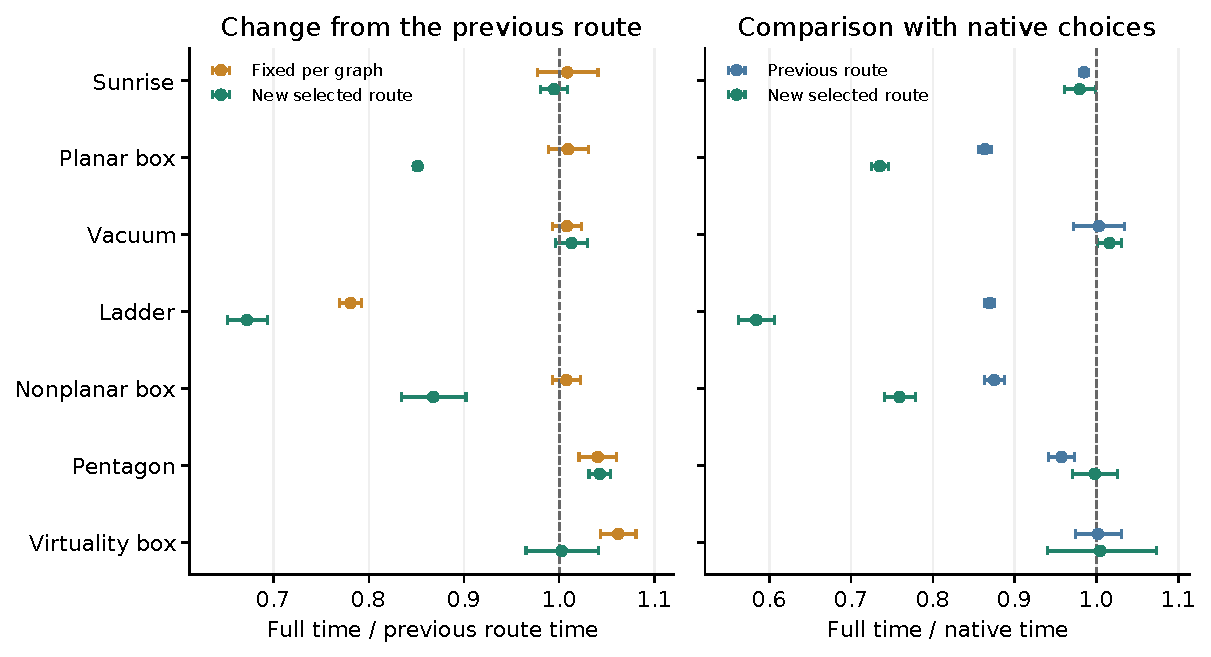
\includegraphics[width=\linewidth]{paper_figures/basis_completion.pdf}
\caption{Selective choices change complete reduction time. Left: the new
fixed strategy and selected method relative to the preceding method.
Right: the preceding and new methods relative to native choices in the
same test. Values below one are faster. Bars show the range over the two
reserved profiles; they are not significance intervals.}
\label{fig:basis-completion}
\end{figure}

\FloatBarrier

The gain is not uniform across the graphs. Relative to the preceding method, the vacuum takes 1.3\% more time, the pentagon 4.3\% more, and the box with external virtuality 0.3\% more. All reported times include prediction, native IBP generation, basis conversion, exact algebra, checks, cleanup, and fallback. These results measure the additional method directly on new parameter profiles; they do not multiply gains from earlier experiments. Their scope remains known graphs and target patterns with rational kinematics, rather than unrestricted symbolic kinematics or arbitrary high-loop scattering.
